% Copyright 2020 by Junwei Wang <i.junwei.wang@gmail.com>
%
% This file may be distributed and/or modified under the
% conditions of the LaTeX Project Public License, either version 1.3c
% of this license or (at your option) any later version.
% The latest version of this license is in
%   http://www.latex-project.org/lppl.txt

% \documentclass[aspectratio=169,compress]{beamer}
\documentclass[aspectratio=169,compress]{beamer}

\usepackage[english]{babel}
\usepackage{metalogo}
\usepackage{listings}
\usepackage{fontspec}
\usepackage{tikz}

% \usetheme{Nord}
\usetheme[style=light]{Nord}


%\usepackage[spanish, es-tabla]{babel}
\usepackage[utf8]{inputenc}
\usepackage{hyperref}




\setmainfont{Yanone Kaffeesatz}
%\setsansfont{Andika New Basic}
\setmonofont{DejaVu Sans Mono}

\setbeamerfont{frametitle}{parent=structure,size=\Large}

\AtBeginSection[]
{
  \begin{frame}[c,noframenumbering,plain]
    \tableofcontents[sectionstyle=show/hide,subsectionstyle=show/show/hide]
  \end{frame}
}

\AtBeginSubsection[]
{
  \begin{frame}[c,noframenumbering,plain]
    \tableofcontents[sectionstyle=show/hide,subsectionstyle=show/shaded/hide]
  \end{frame}
}

\title{Arquitecturas y Organización de Computadoras I}
\subtitle{1: Abstracciones en la computadora y tecnología}
\author{Rafael Ignacio Zurita}
\institute{Depto. Ingeniería de Computadoras}
\date{\today}

\begin{document}

\begin{frame}[plain,noframenumbering]
\bigskip
  \maketitle
\end{frame}

% video
% mostrar varias computadoritas
% mostrar placa con integrados y pcb
% mostrar foto de chip y hablar de los transistores
% mostrar imagen wakerly de transistor CMOS

% imagenes 
% foto de performance
% cuadro python vs C
% foto eras tecnologicas

% historia de ibm
% fotos de computadoras hitos
%     ibm 360 (mainframe), cray1 (supercoputaodra)
%     pdp-11 (creacion de unix) (minicomputadora)
%     4004 primer chip integrado
%     apple II y ibm pc (computadora personal)
%     open mobile komunications (smartphones)
%     iphone smartphone

\section{Abstracciones en la computadora y tecnología}

\subsection{Eras tecnológicas}


\begin{frame}{La computadora: Un sistema complejo}{CHIP}

    \begin{columns}[onlytextwidth,T]
      \column{\dimexpr\linewidth-60mm-5mm}

	\begin{itemize}
	\begin{small}
\bigskip
  \item[Chip] Die en inglés, es empaquetado dentro de un componente que permite su utilizacióin mecánica en un PCB.

\bigskip
\item[Densidad] La tecnología que se utiliza para fabricar los chips (dies), en los circuitos integrados, es el trasistor CMOS.\\
Actualmente la densidad es tan grande que existen miles de millones de transistores en un unico chip.

	\end{small}
	\end{itemize}

      \column{60mm}
    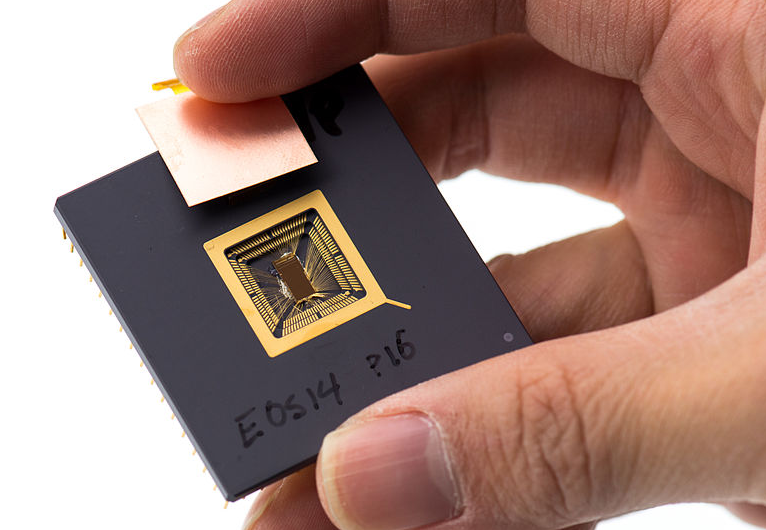
\includegraphics[width=80mm]{images/chip.png}

    \end{columns}
\end{frame}




\begin{frame}{La computadora: Un sistema complejo}{CHIP Barcelona}

    \begin{columns}[onlytextwidth,T]
      \column{\dimexpr\linewidth-60mm-5mm}

	\begin{itemize}
	\begin{small}
\bigskip
  \item[Chip] Die en inglés, es empaquetado dentro de un componente que permite su utilizacióin mecánica en un PCB.

\bigskip
\item[Densidad] La tecnología que se utiliza para fabricar los chips (dies), en los circuitos integrados, es el trasistor CMOS.\\
Actualmente la densidad es tan grande que existen miles de millones de transistores en un unico chip.

\item[Barcelona] Un microprocesador de 4 cores

	\end{small}
	\end{itemize}

      \column{50mm}
    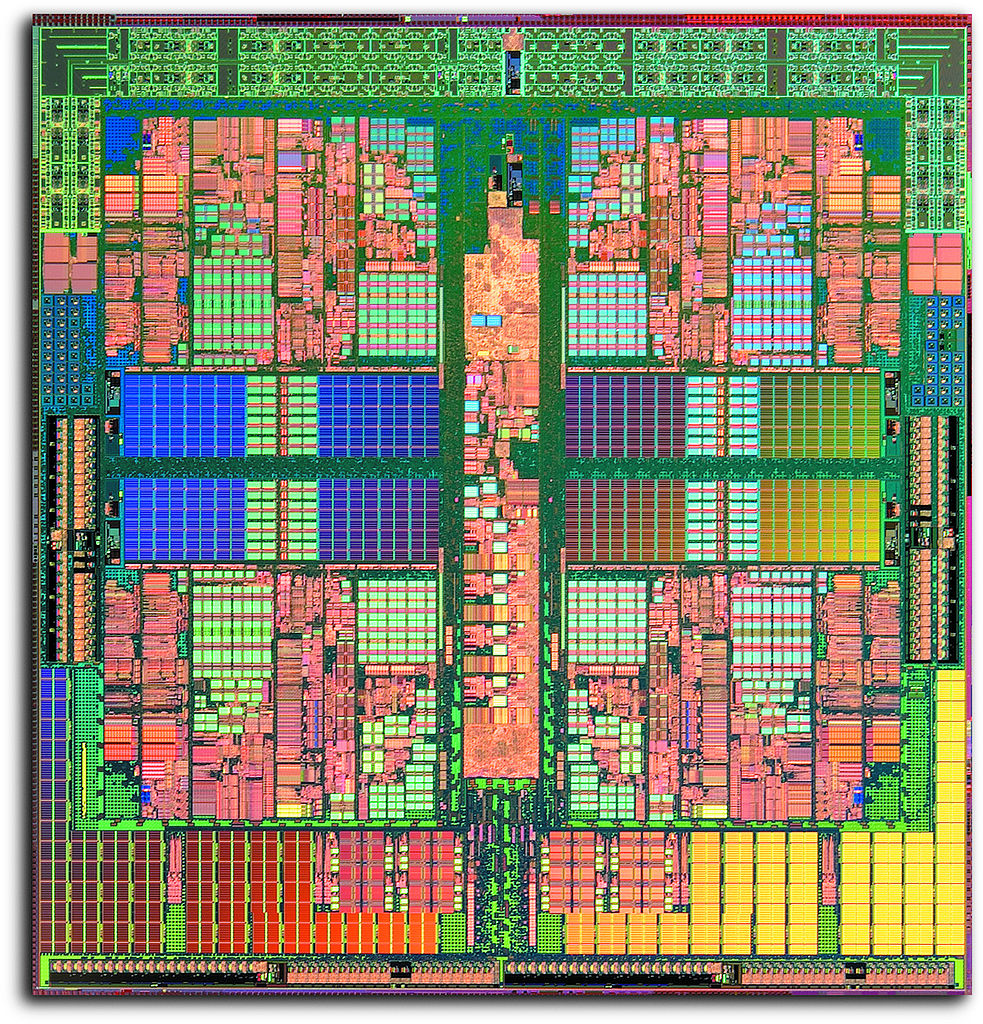
\includegraphics[width=80mm]{images/barcelona.png}

    \end{columns}
\end{frame}


\begin{frame}{La computadora: Un sistema complejo}{Transistor CMOS}

    \begin{columns}[onlytextwidth,T]
      \column{\dimexpr\linewidth-60mm-5mm}

	\begin{itemize}
	\begin{small}
\bigskip
  \item[Compuertas] Con circuitos CMOS se fabrican compuertas, que pueden operar digitalmente y realizar una simple función lógica.

\bigskip
\item[NOT] Una compuerta NOT (circuito básico CMOS) se puede fabricar utilizando dos transistores MOS complementarios.

	\end{small}
	\end{itemize}

      \column{50mm}
    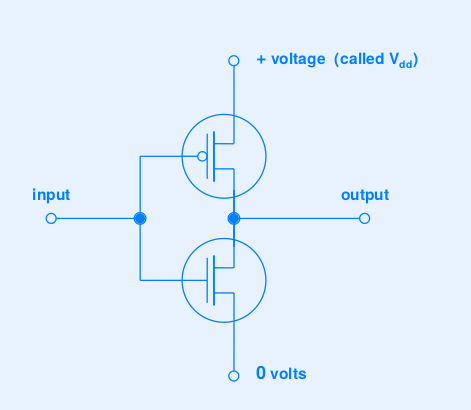
\includegraphics[width=50mm]{images/cmos2.png}

    \end{columns}
\end{frame}



\subsection{Abstracciones en la computadora}


\begin{frame}{La computadora: Un sistema complejo}

    \begin{columns}[onlytextwidth,T]
      \column{\dimexpr\linewidth-60mm-5mm}

	\begin{itemize}
	\begin{small}
\bigskip
  \item[Abstracción] El hardware y software de una computadora
consiste de una jerarquía en capas, donde cada capa de hardware o software
le oculta detalles a la capa superior.

\bigskip

\item[Principio] \textit{El principio de abstracción} es el que \textit{permite}
a los diseñadores de hardware y software poder \textit{entender la complejidad} 
de los sistemas de cómputo que construyen.

\bigskip

\item [Interfaz] EL nivel \textit{Arquitectura del Conjunto de 
Instrucciones (ISA)}, es la interfaz entre el hardware y el software.

	\end{small}
	\end{itemize}

      \column{60mm}
    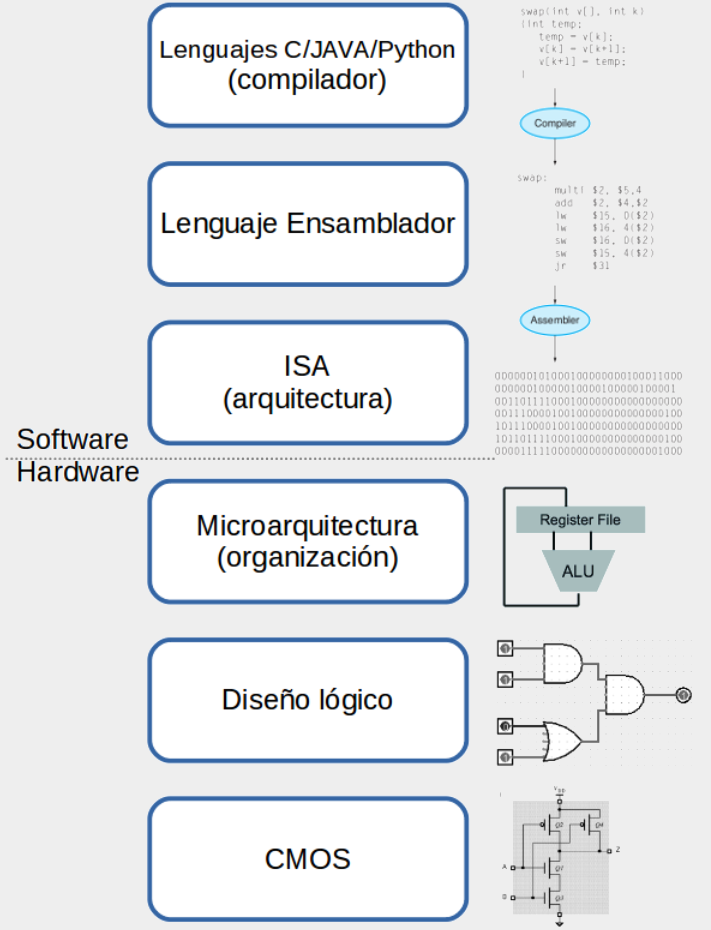
\includegraphics[width=50mm]{images/abstracciones2.png}

    \end{columns}

\end{frame}



\begin{frame} {Diseño lógico} {La computadora: Un sistema complejo}

    \begin{columns}[onlytextwidth,T]
      \column{\dimexpr\linewidth-60mm-5mm}

	\begin{itemize}
	\begin{small}
\bigskip
  \item[Diseño digital] o diseño lógico, es actuamente realizado utilizando el algebra de Boole (también llamado algebra de switching)

  \item[SFM] Las máquinas de estado finito pueden ser esquematizadas con diseño digital, y permitan diseñar máquinas algoritmicas.
\bigskip

	\end{small}
	\end{itemize}

      \column{60mm}
    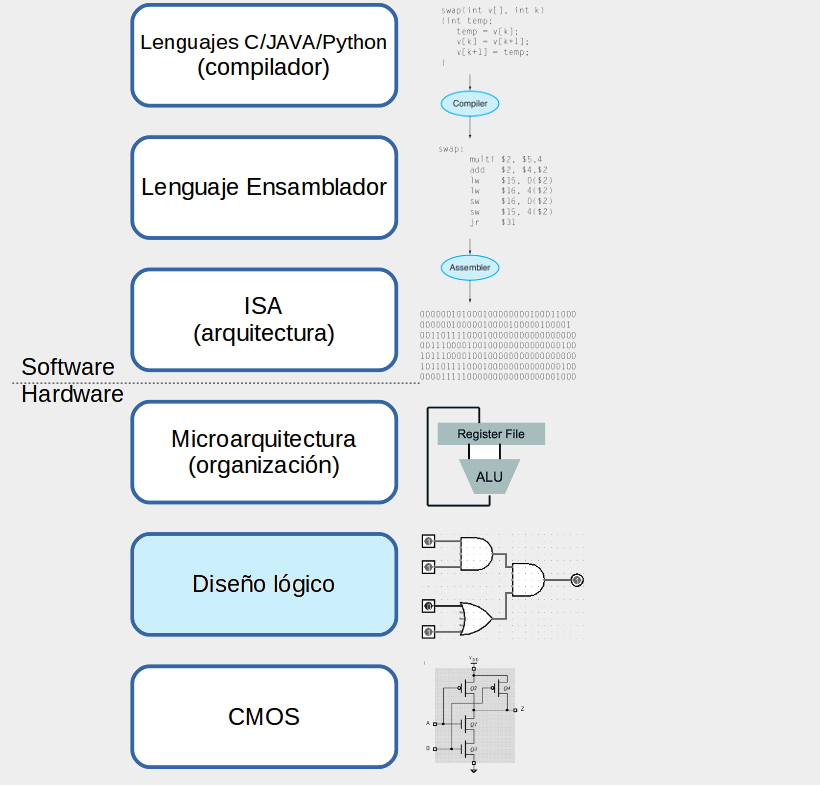
\includegraphics[width=50mm]{images/dis_logico.png}

    \end{columns}

\end{frame}


\begin{frame} {Organización de una computadora} {La computadora: Un sistema complejo}

  \footnotesize{Es el diseño e implementación de la arquitectura (ISA) del microprocesador}

  \begin{columns}[onlytextwidth,T]
      \column{\dimexpr\linewidth-70mm-5mm}

	\begin{itemize}
	\begin{footnotesize}
\item[Micro] Hoy en día, a la organización de una computadora se la conoce como su \textbf{microarquitectura}

\item [Familia] Una arquitectura puede tener muchas organizaciones diferentes. \\

Los fabricantes de microprocesadores modifican regularmente la microarquitectura de un procesador manteniendo su ISA esencialmente constante

\item [Ortogonales] La arquitectura y la organización son ortogonales; es decir, son totalmente independientes


	\end{footnotesize}
	\end{itemize}
\footnotesize{La \textbf{\textit arquitectura} especifica lo \textbf{\textit que} puede hacer una computadora y la \textbf{\textit organización} especifica \textbf{\textit cómo} lo hace.}

      \column{60mm}
	\bigskip
    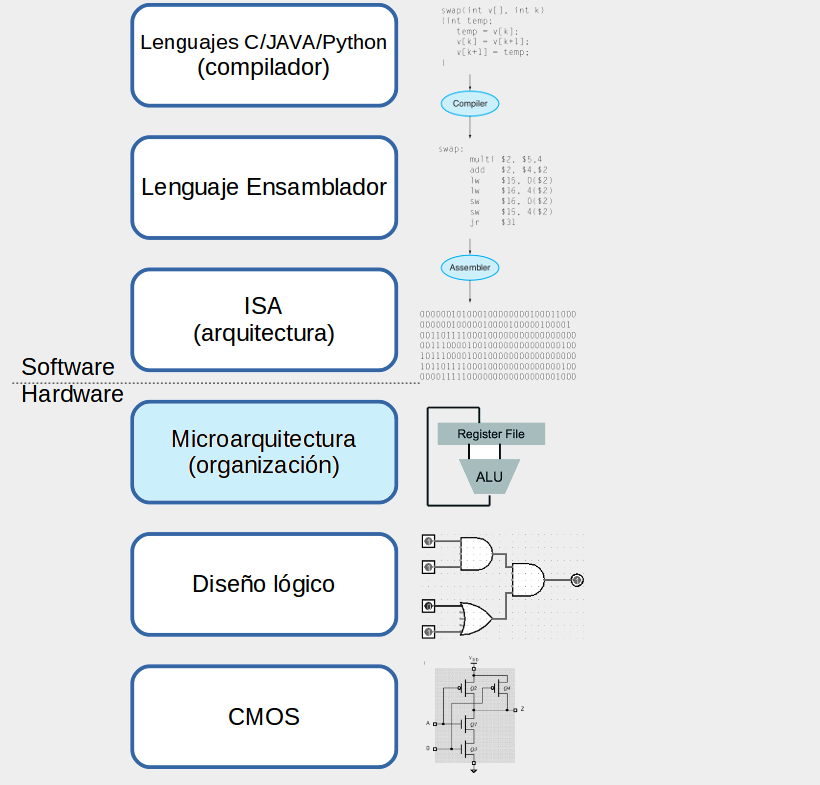
\includegraphics[width=60mm]{images/microarquitectura.png}

    \end{columns}

\end{frame}


\begin{frame}{Arquitectura de una computadora}{La computadora: Un sistema complejo}

  \footnotesize{Es la descripción del lenguaje máquina (arquitectura del conjunto de instrucciones o ISA) \\ de una computadora}

  \begin{columns}[onlytextwidth,T]
      \column{\dimexpr\linewidth-70mm-5mm}

	\begin{itemize}
	\begin{footnotesize}

\item[Modelo] La arquitectura del conjunto de instrucciones define el modelo de programación de una computadora.

\item[Abstracción] La arquitectura es una entidad abstracta, porque no considera detalles específicos del diseño o implementación de una computadora.


\item[Componentes] La arquitectura (ISA) está compuesta por el conjunto de registros del procesador, el conjunto de instrucciones y los modos de direccionamiento.

\item[Interfaz] El lenguaje ensamblador de una computadora (y el programa ensamblador) es una abstracción de la arquitectura

	\end{footnotesize}
	\end{itemize}

      \column{60mm}
	\bigskip
    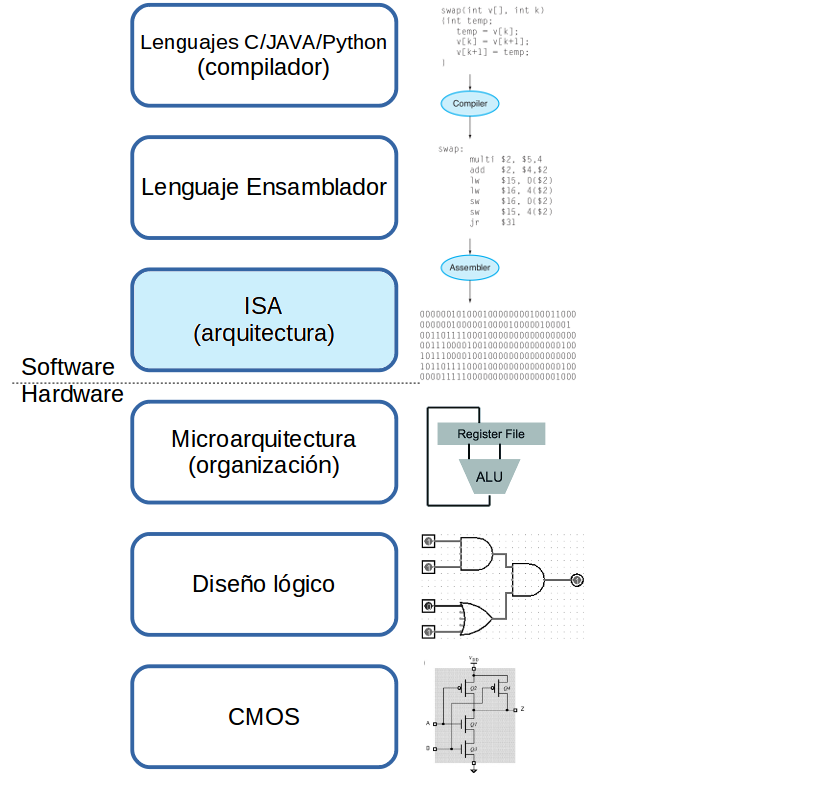
\includegraphics[width=60mm]{images/arquitectura.png}

    \end{columns}

\end{frame}

\subsection{Terminología: Arquitectura y Organización de un procesador}


\subsection{Limitaciones tecnológicas}
\subsection{Tiempo de ejecución (rendimiento)}
\subsection{MIPS/RISCV ISA (Arquitectura de una computadora real)}



\subsection{Recursos}

\begin{frame}[fragile]
  \frametitle{Recursos de la materia}

\begin{small}
\begin{itemize}

\item Web: \footnotesize{\texttt http://se.fi.uncoma.edu.ar/ayod1c/}\\
(se alcanza también desde la materia en PEDCO).

\item FOROs de PEDCO (Novedades y Consultas)
\item Telegram (para consultas)
\item Google meet para las exposiciones y discuciones temáticas online\\ (se darán los enlaces de encuentros en las clases).
\item Bibliografía:

\begin{itemize}

\item Andrew S. Tanenbaum (2000), ORGANIZACIÓN DE COMPUTADORAS un enfoque estructurado, Editorial Prentice Hall. (10 copias en biblioteca)
\item David. Patterson, John L. Hennessy, ORGANIZACIÓN Y DISEÑO DE COMPUTADORES La interfaz hardware/software, McGraw-Hill (8 copias en biblioteca).
\item Apuntes y artículos en la web de la materia
\item David. Patterson, John L. Hennessy, Computer Organization and Design RISC-V Edition 1st Edition The Hardware Software Interface. ISBN: 9780128122754

\end{itemize}

\end{itemize}
\end{small}

\end{frame}


\end{document}

%%% Local Variables:
%%% mode: latex
%%% TeX-master: t
%%% TeX-engine: xetex
%%% End:
